% Options for packages loaded elsewhere
\PassOptionsToPackage{unicode}{hyperref}
\PassOptionsToPackage{hyphens}{url}
%
\documentclass[
]{book}
\usepackage{amsmath,amssymb}
\usepackage{iftex}
\ifPDFTeX
  \usepackage[T1]{fontenc}
  \usepackage[utf8]{inputenc}
  \usepackage{textcomp} % provide euro and other symbols
\else % if luatex or xetex
  \usepackage{unicode-math} % this also loads fontspec
  \defaultfontfeatures{Scale=MatchLowercase}
  \defaultfontfeatures[\rmfamily]{Ligatures=TeX,Scale=1}
\fi
\usepackage{lmodern}
\ifPDFTeX\else
  % xetex/luatex font selection
\fi
% Use upquote if available, for straight quotes in verbatim environments
\IfFileExists{upquote.sty}{\usepackage{upquote}}{}
\IfFileExists{microtype.sty}{% use microtype if available
  \usepackage[]{microtype}
  \UseMicrotypeSet[protrusion]{basicmath} % disable protrusion for tt fonts
}{}
\makeatletter
\@ifundefined{KOMAClassName}{% if non-KOMA class
  \IfFileExists{parskip.sty}{%
    \usepackage{parskip}
  }{% else
    \setlength{\parindent}{0pt}
    \setlength{\parskip}{6pt plus 2pt minus 1pt}}
}{% if KOMA class
  \KOMAoptions{parskip=half}}
\makeatother
\usepackage{xcolor}
\usepackage{color}
\usepackage{fancyvrb}
\newcommand{\VerbBar}{|}
\newcommand{\VERB}{\Verb[commandchars=\\\{\}]}
\DefineVerbatimEnvironment{Highlighting}{Verbatim}{commandchars=\\\{\}}
% Add ',fontsize=\small' for more characters per line
\usepackage{framed}
\definecolor{shadecolor}{RGB}{248,248,248}
\newenvironment{Shaded}{\begin{snugshade}}{\end{snugshade}}
\newcommand{\AlertTok}[1]{\textcolor[rgb]{0.94,0.16,0.16}{#1}}
\newcommand{\AnnotationTok}[1]{\textcolor[rgb]{0.56,0.35,0.01}{\textbf{\textit{#1}}}}
\newcommand{\AttributeTok}[1]{\textcolor[rgb]{0.13,0.29,0.53}{#1}}
\newcommand{\BaseNTok}[1]{\textcolor[rgb]{0.00,0.00,0.81}{#1}}
\newcommand{\BuiltInTok}[1]{#1}
\newcommand{\CharTok}[1]{\textcolor[rgb]{0.31,0.60,0.02}{#1}}
\newcommand{\CommentTok}[1]{\textcolor[rgb]{0.56,0.35,0.01}{\textit{#1}}}
\newcommand{\CommentVarTok}[1]{\textcolor[rgb]{0.56,0.35,0.01}{\textbf{\textit{#1}}}}
\newcommand{\ConstantTok}[1]{\textcolor[rgb]{0.56,0.35,0.01}{#1}}
\newcommand{\ControlFlowTok}[1]{\textcolor[rgb]{0.13,0.29,0.53}{\textbf{#1}}}
\newcommand{\DataTypeTok}[1]{\textcolor[rgb]{0.13,0.29,0.53}{#1}}
\newcommand{\DecValTok}[1]{\textcolor[rgb]{0.00,0.00,0.81}{#1}}
\newcommand{\DocumentationTok}[1]{\textcolor[rgb]{0.56,0.35,0.01}{\textbf{\textit{#1}}}}
\newcommand{\ErrorTok}[1]{\textcolor[rgb]{0.64,0.00,0.00}{\textbf{#1}}}
\newcommand{\ExtensionTok}[1]{#1}
\newcommand{\FloatTok}[1]{\textcolor[rgb]{0.00,0.00,0.81}{#1}}
\newcommand{\FunctionTok}[1]{\textcolor[rgb]{0.13,0.29,0.53}{\textbf{#1}}}
\newcommand{\ImportTok}[1]{#1}
\newcommand{\InformationTok}[1]{\textcolor[rgb]{0.56,0.35,0.01}{\textbf{\textit{#1}}}}
\newcommand{\KeywordTok}[1]{\textcolor[rgb]{0.13,0.29,0.53}{\textbf{#1}}}
\newcommand{\NormalTok}[1]{#1}
\newcommand{\OperatorTok}[1]{\textcolor[rgb]{0.81,0.36,0.00}{\textbf{#1}}}
\newcommand{\OtherTok}[1]{\textcolor[rgb]{0.56,0.35,0.01}{#1}}
\newcommand{\PreprocessorTok}[1]{\textcolor[rgb]{0.56,0.35,0.01}{\textit{#1}}}
\newcommand{\RegionMarkerTok}[1]{#1}
\newcommand{\SpecialCharTok}[1]{\textcolor[rgb]{0.81,0.36,0.00}{\textbf{#1}}}
\newcommand{\SpecialStringTok}[1]{\textcolor[rgb]{0.31,0.60,0.02}{#1}}
\newcommand{\StringTok}[1]{\textcolor[rgb]{0.31,0.60,0.02}{#1}}
\newcommand{\VariableTok}[1]{\textcolor[rgb]{0.00,0.00,0.00}{#1}}
\newcommand{\VerbatimStringTok}[1]{\textcolor[rgb]{0.31,0.60,0.02}{#1}}
\newcommand{\WarningTok}[1]{\textcolor[rgb]{0.56,0.35,0.01}{\textbf{\textit{#1}}}}
\usepackage{longtable,booktabs,array}
\usepackage{calc} % for calculating minipage widths
% Correct order of tables after \paragraph or \subparagraph
\usepackage{etoolbox}
\makeatletter
\patchcmd\longtable{\par}{\if@noskipsec\mbox{}\fi\par}{}{}
\makeatother
% Allow footnotes in longtable head/foot
\IfFileExists{footnotehyper.sty}{\usepackage{footnotehyper}}{\usepackage{footnote}}
\makesavenoteenv{longtable}
\usepackage{graphicx}
\makeatletter
\newsavebox\pandoc@box
\newcommand*\pandocbounded[1]{% scales image to fit in text height/width
  \sbox\pandoc@box{#1}%
  \Gscale@div\@tempa{\textheight}{\dimexpr\ht\pandoc@box+\dp\pandoc@box\relax}%
  \Gscale@div\@tempb{\linewidth}{\wd\pandoc@box}%
  \ifdim\@tempb\p@<\@tempa\p@\let\@tempa\@tempb\fi% select the smaller of both
  \ifdim\@tempa\p@<\p@\scalebox{\@tempa}{\usebox\pandoc@box}%
  \else\usebox{\pandoc@box}%
  \fi%
}
% Set default figure placement to htbp
\def\fps@figure{htbp}
\makeatother
\setlength{\emergencystretch}{3em} % prevent overfull lines
\providecommand{\tightlist}{%
  \setlength{\itemsep}{0pt}\setlength{\parskip}{0pt}}
\setcounter{secnumdepth}{5}
\usepackage{booktabs}
\usepackage{amsthm}
\makeatletter
\def\thm@space@setup{%
  \thm@preskip=8pt plus 2pt minus 4pt
  \thm@postskip=\thm@preskip
}
\makeatother
\usepackage[]{natbib}
\bibliographystyle{apalike}
\usepackage{bookmark}
\IfFileExists{xurl.sty}{\usepackage{xurl}}{} % add URL line breaks if available
\urlstyle{same}
\hypersetup{
  pdftitle={Estadística Multivariada},
  pdfauthor={Haydeé Peruyero},
  hidelinks,
  pdfcreator={LaTeX via pandoc}}

\title{Estadística Multivariada}
\author{Haydeé Peruyero}
\date{}

\begin{document}
\maketitle

{
\setcounter{tocdepth}{1}
\tableofcontents
}
\chapter{Estadística Multivariada}\label{estaduxedstica-multivariada}

\section{Temario}\label{temario}

\begin{enumerate}
\def\labelenumi{\arabic{enumi}.}
\tightlist
\item
  Regresión múltiple
\end{enumerate}

1.1 Mínimos cuadrados.

1.2 Medidas de bondad de ajuste.

1.3 Determinación del número de variables predictorias.

\begin{enumerate}
\def\labelenumi{\arabic{enumi}.}
\setcounter{enumi}{1}
\tightlist
\item
  Análisis de componentes principales
\end{enumerate}

2.1 Descripción de la metodología.

2.2 Técnicas de extracción de componentes principales.

2.3 Determinación del número de componentes principales.

\begin{enumerate}
\def\labelenumi{\arabic{enumi}.}
\setcounter{enumi}{2}
\tightlist
\item
  Análisis factorial
\end{enumerate}

3.1 Descripción de la metodología del análisis factorial.

3.2 Descripción del modelo básico.

3.3 Método de cálculo.

3.4 Comparación con la técnica del análisis de componentes principales.

3.5 Usos de software (R, Minitab, SciPy, entre otros).

\begin{enumerate}
\def\labelenumi{\arabic{enumi}.}
\setcounter{enumi}{3}
\tightlist
\item
  Análisis de conglomerados
\end{enumerate}

4.1Descripción de la metodología de análisis de conglomerados.

4.2 Técnicas de jerarquización y de particionamiento.

4.3 Implementación computacional.

4.4 Usos de los dendogramas.

4.5 Usos de software (R, Minitab, SciPy, entre otros).

\begin{enumerate}
\def\labelenumi{\arabic{enumi}.}
\setcounter{enumi}{4}
\tightlist
\item
  Análisis discriminante
\end{enumerate}

5.1 Descripción de la metodología del análisis discriminante.

5.2 Discriminación entre dos grupos.

5.3 Contribución por variable.

5.4 Discriminación logística.

5.5 Discriminación múltiple.

5.6 Usos de software (R, Minitab, SciPy, entre otros).

A1. R

A2. Git + Github

A3. Gráficas Multivariadas

A4. Escalas de Medición

A5. Valores Faltantes

\section{Evaluación}\label{evaluaciuxf3n}

\begin{itemize}
\tightlist
\item
  Examenes 50\%
\item
  Tareas 25\%
\item
  Proyecto 20\%
\item
  DataCamp 5\%
\end{itemize}

\section{Proyecto final}\label{proyecto-final}

\begin{itemize}
\tightlist
\item
  Buscar una base de datos ``real''
\item
  Aplicar 3 métodos de estadística multivariada
\item
  Entregar documento con:

  \begin{itemize}
  \tightlist
  \item
    Descripción de los datos
  \item
    Planteamiento del problema
  \item
    Métodos usados
  \item
    Interpretación de resultados
  \item
    Código usado
  \end{itemize}
\item
  Repositorio con código reproducible
\item
  Exposición de resultados
\end{itemize}

\section{Referencias}\label{referencias}

{[}1{]}

\section{Material interesante}\label{material-interesante}

\begin{itemize}
\tightlist
\item
  \href{https://bookdown.org/}{Bookdown}.
\item
  \href{https://swcarpentry.github.io/r-novice-gapminder/}{Software Carpentry}.
\item
  \href{https://swcarpentry.github.io/git-novice/14-supplemental-rstudio/}{Git}
\item
  \href{https://info5940.infosci.cornell.edu/setup/git/what-is-git/}{Why Git}
\item
  \href{https://bookdown.org/yihui/rmarkdown-cookbook/}{R Markdown Cookbook}
\item
  \href{http://www.sthda.com/english/wiki/data-visualization}{STHDA}
\item
  \href{https://bookdown.org/ndphillips/YaRrr/}{YaRrr! The Pirate's Guide to R}
\item
  \href{https://link.springer.com/book/10.1007/978-3-319-53019-2}{Learn ggplot2 Using Shiny App}
\item
  \href{https://link.springer.com/book/10.1007/978-0-387-98141-3}{Ggplot2: Elegant Graphics for Data Analysis}

  \begin{itemize}
  \tightlist
  \item
    \href{https://ggplot2-book.org/index.html}{Versión online}
  \end{itemize}
\item
  \href{https://www.springer.com/series/6991/books}{Use R! Colección Springer}
\item
  \href{https://link.springer.com/book/10.1007/978-0-387-75969-2}{Lattice: Multivariate Data Visualization with R}
\item
  \href{http://www.cookbook-r.com/}{R Graphics cookbook}
\item
  \href{https://education.github.com/benefits}{Cuenta pro de Github}
\end{itemize}

\section{DataCamp}\label{datacamp}

\begin{figure}
\centering
\pandocbounded{
\includegraphics[keepaspectratio]{img/regular.png}}
\caption{DataCamp}
\end{figure}

\chapter{Regresión múltiple}\label{regresiuxf3n-muxfaltiple}

\section{¿Por qué estadística multivariada?}\label{por-quuxe9-estaduxedstica-multivariada}

El proceso de modelado consiste en construir expresiones matemáticas que permitan representar el comportamiento de una variable que queremos estudiar. Cuando contamos con varias variables, suele interesarnos analizar cómo unas influyen sobre otras, determinando si existe una relación, su intensidad y su forma. En muchos casos, estas relaciones pueden ser complejas y difíciles de describir directamente; por ello, se busca aproximarlas mediante funciones matemáticas sencillas como polinomios, que conserven los elementos esenciales para explicar el fenómeno de interés.

Cuando estudiamos fenómenos deterministas, es común vincular una variable dependiente con una o más variables independientes. Por ejemplo, en la ecuación de la velocidad (\(v=d/t\)), la distancia depende de la velocidad y del tiempo. En la práctica, cuando realizamos distintos experimentos, las fórmulas deterministas podrían no capturar por completo el comportamiento observado. Esto puede deberse a factores no controlados, a la presencia de variabilidad natural o a efectos aleatorios. Por esta razón, además de la parte determinista del modelo, se incorpora un término que represente la discrepancia aleatoria entre lo que se predice y lo que efectivamente se observa. De forma general, esta idea se resume como:

\[Observación = Modelo \ + \ Error\]

Cuando se supone que la relación entre las variables puede representarse mediante una ecuación lineal, hablamos de \emph{análisis de regresión lineal}. Si intervienen únicamente dos variables, una dependiente \(y\) y independiente \(x\), se trata de \textbf{regresión lineal simple}. En cambio, cuando la variable de interés \(y\) depende de dos o más variables independientes \(x_1,x_2, ...\) hablamos de \textbf{regresión lineal múltiple}.

\emph{Supongamos que queremos predecir el rendimiento académico de un estudiante, ¿solo necesitamos las horas que estudia?}

En este caso se tiene que el puntaje o rendimiento lo podemos representar con \(y\) y las horas de estudio con \(x\). Entonces esta propuesta de modelo, la podríamos representar como:

\[y=\beta_0+\beta_1x\]
Donde \(\beta_0\) es la ordenada al origen y \(\beta_1\) la pendiente. Esta recta podría no ajustarse al modelo por diferentes razones, entonces lo que se hace es considerar un error aleatorio \(\epsilon\). El modelo que ya considera este error se representa como:

\[y=\beta_0+\beta_1x+\epsilon.\]

A este modelo se le conoce como modelo de \textbf{regresión lineal simple} y a \(\beta_0,\beta_1\) se les conoce como \textbf{coeficientes de regresión}.

En problemas reales, casi nunca una sola variable explica el fenómeno. Las decisiones y predicciones mejoran cuando integramos múltiples fuentes de información.

Ejemplos:
- Salud: riesgo de una enfermedad según edad, IMC, actividad física, dieta y antecedentes.
- Ingeniería: vida útil de una pieza según temperatura, vibración, material y carga.
- Biología: crecimiento de una planta por agua, luz, fertilizante, temperatura.

\textbf{Ejemplo:} Si queremos predecir el rendimiento académico de un estudiante, ¿solo necesitamos las horas que estudia? ¿qué otras variables podrían influir en el puntaje de un examen?

Rendimiento escolar

\begin{Shaded}
\begin{Highlighting}[]
\FunctionTok{set.seed}\NormalTok{(}\DecValTok{123}\NormalTok{)}
\NormalTok{n }\OtherTok{\textless{}{-}} \DecValTok{10}
\NormalTok{data\_intro }\OtherTok{\textless{}{-}} \FunctionTok{tibble}\NormalTok{(}
  \AttributeTok{estudiante =} \FunctionTok{paste0}\NormalTok{(}\StringTok{"E"}\NormalTok{, }\DecValTok{1}\SpecialCharTok{:}\NormalTok{n),}
  \AttributeTok{horas\_estudio =} \FunctionTok{c}\NormalTok{(}\DecValTok{2}\NormalTok{,}\DecValTok{3}\NormalTok{,}\DecValTok{4}\NormalTok{,}\DecValTok{5}\NormalTok{,}\DecValTok{1}\NormalTok{,}\DecValTok{3}\NormalTok{,}\DecValTok{2}\NormalTok{,}\DecValTok{4}\NormalTok{,}\DecValTok{5}\NormalTok{,}\DecValTok{6}\NormalTok{),}
  \AttributeTok{horas\_sueno  =} \FunctionTok{c}\NormalTok{(}\DecValTok{7}\NormalTok{,}\DecValTok{8}\NormalTok{,}\DecValTok{6}\NormalTok{,}\DecValTok{7}\NormalTok{,}\DecValTok{5}\NormalTok{,}\DecValTok{8}\NormalTok{,}\DecValTok{7}\NormalTok{,}\DecValTok{6}\NormalTok{,}\DecValTok{9}\NormalTok{,}\DecValTok{7}\NormalTok{),}
  \AttributeTok{asistencia   =} \FunctionTok{c}\NormalTok{(}\FloatTok{0.9}\NormalTok{,}\FloatTok{0.95}\NormalTok{,}\FloatTok{0.8}\NormalTok{,}\FloatTok{0.85}\NormalTok{,}\FloatTok{0.7}\NormalTok{,}\FloatTok{0.9}\NormalTok{,}\FloatTok{0.8}\NormalTok{,}\FloatTok{0.9}\NormalTok{,}\DecValTok{1}\NormalTok{,}\FloatTok{0.95}\NormalTok{),}
  \AttributeTok{puntaje      =} \FunctionTok{c}\NormalTok{(}\DecValTok{65}\NormalTok{,}\DecValTok{70}\NormalTok{,}\DecValTok{68}\NormalTok{,}\DecValTok{80}\NormalTok{,}\DecValTok{60}\NormalTok{,}\DecValTok{75}\NormalTok{,}\DecValTok{65}\NormalTok{,}\DecValTok{78}\NormalTok{,}\DecValTok{88}\NormalTok{,}\DecValTok{85}\NormalTok{)}
\NormalTok{)}
\NormalTok{data\_intro}
\end{Highlighting}
\end{Shaded}

\begin{verbatim}
## # A tibble: 10 x 5
##    estudiante horas_estudio horas_sueno asistencia puntaje
##    <chr>              <dbl>       <dbl>      <dbl>   <dbl>
##  1 E1                     2           7       0.9       65
##  2 E2                     3           8       0.95      70
##  3 E3                     4           6       0.8       68
##  4 E4                     5           7       0.85      80
##  5 E5                     1           5       0.7       60
##  6 E6                     3           8       0.9       75
##  7 E7                     2           7       0.8       65
##  8 E8                     4           6       0.9       78
##  9 E9                     5           9       1         88
## 10 E10                    6           7       0.95      85
\end{verbatim}

¿Qué pasa si solo graficamos horas de estudio vs puntaje?

Plot hotas de estudio vs puntaje sugerida

\begin{Shaded}
\begin{Highlighting}[]
\FunctionTok{library}\NormalTok{(ggplot2)}
\FunctionTok{ggplot}\NormalTok{(data\_intro, }\FunctionTok{aes}\NormalTok{(horas\_estudio, puntaje)) }\SpecialCharTok{+}
  \FunctionTok{geom\_point}\NormalTok{(}\AttributeTok{size=}\DecValTok{3}\NormalTok{) }\SpecialCharTok{+}
  \FunctionTok{geom\_smooth}\NormalTok{(}\AttributeTok{method=}\StringTok{"lm"}\NormalTok{, }\AttributeTok{se=}\ConstantTok{FALSE}\NormalTok{) }\SpecialCharTok{+}
  \FunctionTok{labs}\NormalTok{(}\AttributeTok{title=}\StringTok{"¿Solo horas de estudio explican el puntaje?"}\NormalTok{)}
\end{Highlighting}
\end{Shaded}

\begin{verbatim}
## `geom_smooth()` using formula = 'y ~ x'
\end{verbatim}

\pandocbounded{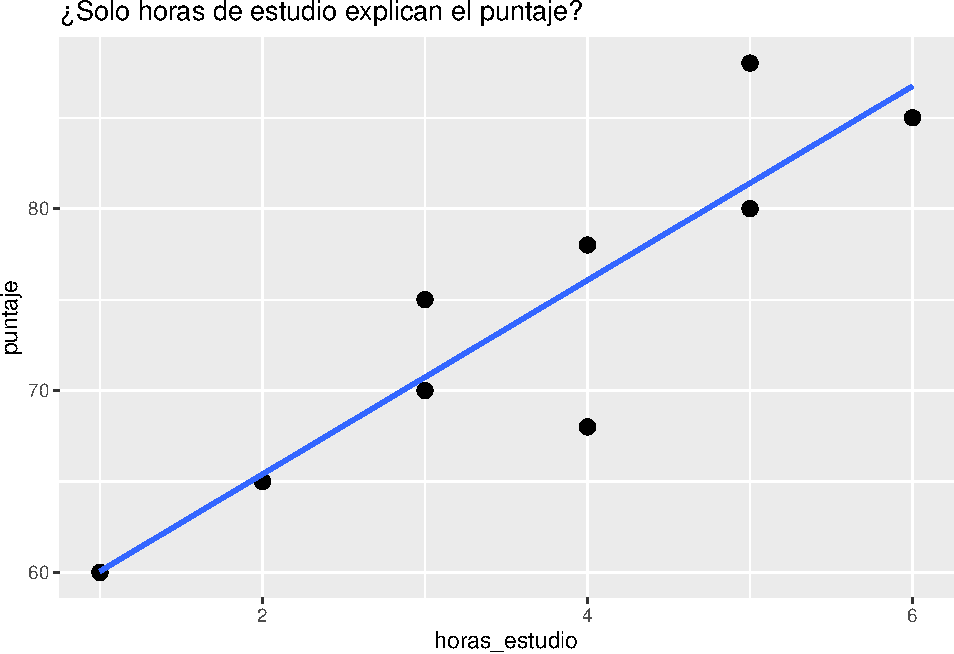
\includegraphics[keepaspectratio]{MultivariateStatisticalAnalysis_files/figure-latex/unnamed-chunk-3-1.pdf}}

¿Se ajusta un modelo lineal? ¿Porqué?

\subsection{¿Qué es ``multivariado'' y por qué lo necesitamos?}\label{quuxe9-es-multivariado-y-por-quuxe9-lo-necesitamos}

\textbf{Idea central:} cuando \textbf{varias} \(x\) influyen sobre \(y\), estudiar cada \(x\) por separado puede engañarnos. El análisis multivariado permite:

\begin{itemize}
\tightlist
\item
  \textbf{Aislar efectos}: estimar el efecto de \(x_1\) \emph{manteniendo constantes} \(x_2,x_3,...\).
\item
  \textbf{Mejorar predicción}: reducir error al añadir información relevante.
\item
  \textbf{Controlar confusores}: variables que cambian la relación aparente entre \(y\) y \(x\).
\end{itemize}

\textbf{Ejemplo:} Si ajustamos ahora un modelo con varias variables, ¿vamos a observar un cambio? ¿se ajustará mejor?

Código (modelos + comparaciones)

\begin{Shaded}
\begin{Highlighting}[]
\CommentTok{\# Modelo simple}
\NormalTok{m1 }\OtherTok{\textless{}{-}} \FunctionTok{lm}\NormalTok{(puntaje }\SpecialCharTok{\textasciitilde{}}\NormalTok{ horas\_estudio, }\AttributeTok{data =}\NormalTok{ data\_intro)}

\CommentTok{\# Modelo múltiple}
\NormalTok{m2 }\OtherTok{\textless{}{-}} \FunctionTok{lm}\NormalTok{(puntaje }\SpecialCharTok{\textasciitilde{}}\NormalTok{ horas\_estudio }\SpecialCharTok{+}\NormalTok{ horas\_sueno }\SpecialCharTok{+}\NormalTok{ asistencia, }\AttributeTok{data =}\NormalTok{ data\_intro)}

\CommentTok{\# Medidas clave}
\NormalTok{R2\_m1  }\OtherTok{\textless{}{-}} \FunctionTok{glance}\NormalTok{(m1)}\SpecialCharTok{$}\NormalTok{r.squared}
\NormalTok{R2\_m2  }\OtherTok{\textless{}{-}} \FunctionTok{glance}\NormalTok{(m2)}\SpecialCharTok{$}\NormalTok{r.squared}

\FunctionTok{print}\NormalTok{(}\FunctionTok{paste}\NormalTok{(}\StringTok{"El R2 del modelo simple:"}\NormalTok{, R2\_m1))}
\end{Highlighting}
\end{Shaded}

\begin{verbatim}
## [1] "El R2 del modelo simple: 0.824317362184441"
\end{verbatim}

\begin{Shaded}
\begin{Highlighting}[]
\FunctionTok{print}\NormalTok{(}\FunctionTok{paste}\NormalTok{(}\StringTok{"El R2 del modelo multiple:"}\NormalTok{, R2\_m2))}
\end{Highlighting}
\end{Shaded}

\begin{verbatim}
## [1] "El R2 del modelo multiple: 0.895428180549875"
\end{verbatim}

\begin{Shaded}
\begin{Highlighting}[]
\CommentTok{\#R2adj\_m1 \textless{}{-} glance(m1)$adj.r.squared}
\CommentTok{\#R2adj \_m2 \textless{}{-} glance(m2)$adj.r.squared}
\end{Highlighting}
\end{Shaded}

\begin{itemize}
\tightlist
\item
  ¿Aumentó \(R^2\) al incluir más variables? ¿Por qué tiende a subir?
\item
  ¿Qué cambia en la interpretación de horas\_estudio al controlar por horas\_sueno y asistencia?
\item
  ¿Puede un predictor ser importante en bivariado y no en multivariado (o viceversa)?
\end{itemize}

\section{Regresión múltiple}\label{regresiuxf3n-muxfaltiple-1}

\subsection{Modelo y estimación}\label{modelo-y-estimaciuxf3n}

Los modelos en regresión lineal múltiple están dados por la siguiente forma, donde \(y\) depende de \(p\) variables predictoras:

\[y_i=\beta_0+\beta_1x_{i1}+\beta_2x_{i2} + \beta_px_{ip}+\epsilon_i.\]

Se suele asumir que los errores \(\epsilon_i\) son i.i.d. con distribución normal de media 0 y varianza \(\sigma^2\) desconocida. Los coeficientes \(\beta_i\) son constantes desconocidas y son los parámetros del modelo. Cada \(\beta_j\) representa el cambio esperado en la respuesta \(y\) por el cambio unitario en \(x_i\) cuando todas las demás variables independientes \(x_i(i\neq j)\) se mantienen constantes.

\begin{Shaded}
\begin{Highlighting}[]
\CommentTok{\# Forma general}
\NormalTok{ajuste }\OtherTok{\textless{}{-}} \FunctionTok{lm}\NormalTok{(y }\SpecialCharTok{\textasciitilde{}}\NormalTok{ x1 }\SpecialCharTok{+}\NormalTok{ x2 }\SpecialCharTok{+}\NormalTok{ ... }\SpecialCharTok{+}\NormalTok{ xp, }\AttributeTok{data =}\NormalTok{ datos)}
\CommentTok{\# summary(ajuste)}
\end{Highlighting}
\end{Shaded}

Los coeficientes los podemos interpretar como sigue:

\begin{itemize}
\tightlist
\item
  \textbf{Intercepto (\(\beta_0\))}: valor esperado de \(y\) cuando todas las \(x\)=0.
\item
  \textbf{Pendiente \(\beta_j\)}: efecto \textbf{parcial} de \(x_j\) sobre \(y\) manteniendo las demás constantes.
\end{itemize}

En los modelos de regreción lineal, solemos usar las siguientes medidas de bondad de ajuste:

\begin{itemize}
\tightlist
\item
  \textbf{\(R^2\)}: proporción de varianza de \(y\) explicada.
\item
  \textbf{\(R^2\) ajustado}: penaliza por número de predictores (mejor para comparar modelos con distinto número de x).
\item
  \textbf{RMSE (\(\sigma\))}: error típico de predicción en unidades de \(y\).
\end{itemize}

\begin{Shaded}
\begin{Highlighting}[]
\NormalTok{comp }\OtherTok{\textless{}{-}}\NormalTok{ dplyr}\SpecialCharTok{::}\FunctionTok{bind\_rows}\NormalTok{(}
  \FunctionTok{glance}\NormalTok{(m1) }\SpecialCharTok{\%\textgreater{}\%} \FunctionTok{mutate}\NormalTok{(}\AttributeTok{modelo=}\StringTok{"simple"}\NormalTok{),}
  \FunctionTok{glance}\NormalTok{(m2) }\SpecialCharTok{\%\textgreater{}\%} \FunctionTok{mutate}\NormalTok{(}\AttributeTok{modelo=}\StringTok{"multiple"}\NormalTok{)}
\NormalTok{) }\SpecialCharTok{\%\textgreater{}\%} \FunctionTok{select}\NormalTok{(modelo, r.squared, adj.r.squared)}
\NormalTok{comp}
\end{Highlighting}
\end{Shaded}

\begin{verbatim}
## # A tibble: 2 x 3
##   modelo   r.squared adj.r.squared
##   <chr>        <dbl>         <dbl>
## 1 simple       0.824         0.802
## 2 multiple     0.895         0.843
\end{verbatim}

Para este modelo algunos de los supuestos se siguen del modelo de regresión lineal
simple y se agregan algunos que tienen que ver con la relación que pudiera existir entre
las variables regresoras.

\begin{itemize}
\tightlist
\item
  El modelo es lineal en los parámetros.\\
  \emph{Chequeo}: residuales vs ajustados sin patrón claro.
\item
  El modelo está especificado correctamente.
\item
  Covarianza cero entre variables regresoras y el error.
\item
  Esperanza del error igual a cero.
\item
  Homocedasticidad.
\item
  No autocorrelación entre los errores.
\item
  Los errores siguen una distribución normal.
\item
  Mas observaciones que parámetros a estimar.
\item
  Variación entre los valores de las variables regresoras.
\item
  No colinealidad (multicolinealidad) entre las variables regresoras, es decir, no existe
  una relación lineal entre \(x_i\) y \(x_j\) (es decir, las variables son linealmente independientes).
\end{itemize}

Supuestos

\begin{Shaded}
\begin{Highlighting}[]
\CommentTok{\# Modelo m2}
\FunctionTok{par}\NormalTok{(}\AttributeTok{mfrow=}\FunctionTok{c}\NormalTok{(}\DecValTok{1}\NormalTok{,}\DecValTok{2}\NormalTok{))}
\FunctionTok{plot}\NormalTok{(m2, }\AttributeTok{which=}\DecValTok{1}\NormalTok{)  }\CommentTok{\# Residuales vs ajustados}
\FunctionTok{plot}\NormalTok{(m2, }\AttributeTok{which=}\DecValTok{2}\NormalTok{)  }\CommentTok{\# QQ{-}plot}
\end{Highlighting}
\end{Shaded}

\pandocbounded{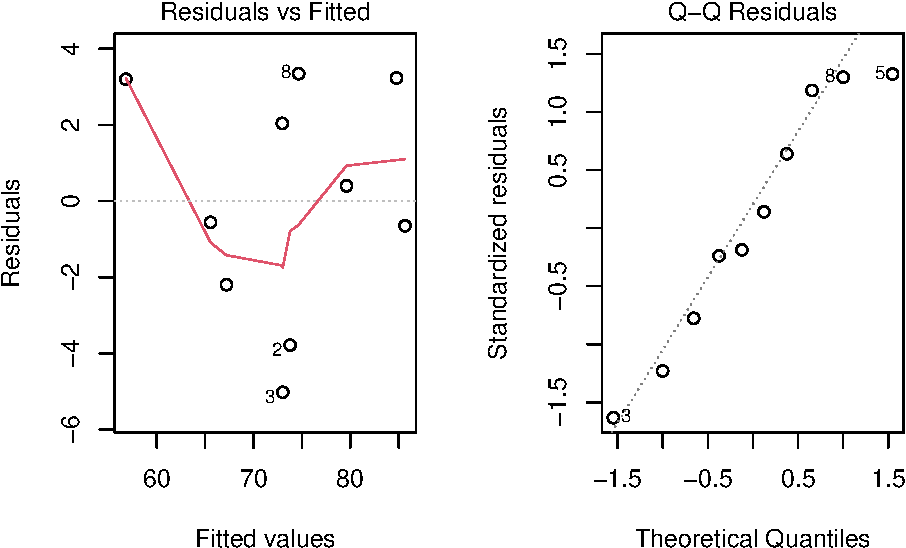
\includegraphics[keepaspectratio]{MultivariateStatisticalAnalysis_files/figure-latex/unnamed-chunk-7-1.pdf}}

\begin{center}\rule{0.5\linewidth}{0.5pt}\end{center}

\textbf{Ejercicio}: Supongamos que tenemos los siguientes datos: precio de vivienda según metros, habitaciones y distancia al centro.

Dataset

\begin{Shaded}
\begin{Highlighting}[]
\FunctionTok{set.seed}\NormalTok{(}\DecValTok{42}\NormalTok{)}
\NormalTok{n }\OtherTok{\textless{}{-}} \DecValTok{14}
\NormalTok{casas }\OtherTok{\textless{}{-}}\NormalTok{ tibble}\SpecialCharTok{::}\FunctionTok{tibble}\NormalTok{(}
  \AttributeTok{precio =} \FunctionTok{c}\NormalTok{(}\DecValTok{200}\NormalTok{,}\DecValTok{220}\NormalTok{,}\DecValTok{250}\NormalTok{,}\DecValTok{275}\NormalTok{,}\DecValTok{300}\NormalTok{,}\DecValTok{180}\NormalTok{,}\DecValTok{210}\NormalTok{,}\DecValTok{260}\NormalTok{,}\DecValTok{280}\NormalTok{,}\DecValTok{320}\NormalTok{,}\DecValTok{190}\NormalTok{,}\DecValTok{240}\NormalTok{,}\DecValTok{230}\NormalTok{,}\DecValTok{305}\NormalTok{),}
  \AttributeTok{metros =} \FunctionTok{c}\NormalTok{(}\DecValTok{80}\NormalTok{,}\DecValTok{90}\NormalTok{,}\DecValTok{100}\NormalTok{,}\DecValTok{110}\NormalTok{,}\DecValTok{120}\NormalTok{,}\DecValTok{70}\NormalTok{,}\DecValTok{85}\NormalTok{,}\DecValTok{105}\NormalTok{,}\DecValTok{115}\NormalTok{,}\DecValTok{130}\NormalTok{,}\DecValTok{75}\NormalTok{,}\DecValTok{95}\NormalTok{,}\DecValTok{92}\NormalTok{,}\DecValTok{125}\NormalTok{),}
  \AttributeTok{habitaciones =} \FunctionTok{c}\NormalTok{(}\DecValTok{2}\NormalTok{,}\DecValTok{3}\NormalTok{,}\DecValTok{3}\NormalTok{,}\DecValTok{4}\NormalTok{,}\DecValTok{4}\NormalTok{,}\DecValTok{2}\NormalTok{,}\DecValTok{3}\NormalTok{,}\DecValTok{3}\NormalTok{,}\DecValTok{4}\NormalTok{,}\DecValTok{5}\NormalTok{,}\DecValTok{2}\NormalTok{,}\DecValTok{3}\NormalTok{,}\DecValTok{3}\NormalTok{,}\DecValTok{4}\NormalTok{),}
  \AttributeTok{distancia\_centro =} \FunctionTok{c}\NormalTok{(}\DecValTok{5}\NormalTok{,}\DecValTok{4}\NormalTok{,}\DecValTok{6}\NormalTok{,}\DecValTok{3}\NormalTok{,}\DecValTok{2}\NormalTok{,}\DecValTok{8}\NormalTok{,}\DecValTok{6}\NormalTok{,}\DecValTok{3}\NormalTok{,}\DecValTok{2}\NormalTok{,}\DecValTok{1}\NormalTok{,}\DecValTok{7}\NormalTok{,}\DecValTok{5}\NormalTok{,}\DecValTok{4}\NormalTok{,}\DecValTok{2}\NormalTok{)}
\NormalTok{)}
\NormalTok{casas}
\end{Highlighting}
\end{Shaded}

\begin{verbatim}
## # A tibble: 14 x 4
##    precio metros habitaciones distancia_centro
##     <dbl>  <dbl>        <dbl>            <dbl>
##  1    200     80            2                5
##  2    220     90            3                4
##  3    250    100            3                6
##  4    275    110            4                3
##  5    300    120            4                2
##  6    180     70            2                8
##  7    210     85            3                6
##  8    260    105            3                3
##  9    280    115            4                2
## 10    320    130            5                1
## 11    190     75            2                7
## 12    240     95            3                5
## 13    230     92            3                4
## 14    305    125            4                2
\end{verbatim}

\begin{enumerate}
\def\labelenumi{\arabic{enumi})}
\tightlist
\item
  Ajusta \texttt{precio\ \textasciitilde{}\ metros} (simple) y \texttt{precio\ \textasciitilde{}\ metros\ +\ habitaciones\ +\ distancia\_centro} (múltiple).\\
\item
  Compara \(R^2\), \(R^2\) \textbf{ajustado} y \textbf{σ (RMSE)}.\\
\item
  Interpreta el coeficiente de \texttt{distancia\_centro}.\\
\item
  Revisa QQ-plot y residuales vs ajustados. ¿Algún patrón?
\end{enumerate}

Solución

\begin{Shaded}
\begin{Highlighting}[]
\NormalTok{m\_s }\OtherTok{\textless{}{-}} \FunctionTok{lm}\NormalTok{(precio }\SpecialCharTok{\textasciitilde{}}\NormalTok{ metros, }\AttributeTok{data=}\NormalTok{casas)}
\NormalTok{m\_m }\OtherTok{\textless{}{-}} \FunctionTok{lm}\NormalTok{(precio }\SpecialCharTok{\textasciitilde{}}\NormalTok{ metros }\SpecialCharTok{+}\NormalTok{ habitaciones }\SpecialCharTok{+}\NormalTok{ distancia\_centro, }\AttributeTok{data=}\NormalTok{casas)}

\NormalTok{broom}\SpecialCharTok{::}\FunctionTok{glance}\NormalTok{(m\_s)[,}\FunctionTok{c}\NormalTok{(}\StringTok{"r.squared"}\NormalTok{,}\StringTok{"adj.r.squared"}\NormalTok{)]}
\end{Highlighting}
\end{Shaded}

\begin{verbatim}
## # A tibble: 1 x 2
##   r.squared adj.r.squared
##       <dbl>         <dbl>
## 1     0.996         0.996
\end{verbatim}

\begin{Shaded}
\begin{Highlighting}[]
\NormalTok{broom}\SpecialCharTok{::}\FunctionTok{glance}\NormalTok{(m\_m)[,}\FunctionTok{c}\NormalTok{(}\StringTok{"r.squared"}\NormalTok{,}\StringTok{"adj.r.squared"}\NormalTok{)]}
\end{Highlighting}
\end{Shaded}

\begin{verbatim}
## # A tibble: 1 x 2
##   r.squared adj.r.squared
##       <dbl>         <dbl>
## 1     0.997         0.996
\end{verbatim}

\begin{Shaded}
\begin{Highlighting}[]
\NormalTok{broom}\SpecialCharTok{::}\FunctionTok{tidy}\NormalTok{(m\_m)}
\end{Highlighting}
\end{Shaded}

\begin{verbatim}
## # A tibble: 4 x 5
##   term             estimate std.error statistic      p.value
##   <chr>               <dbl>     <dbl>     <dbl>        <dbl>
## 1 (Intercept)        -8.67     14.9      -0.583 0.573       
## 2 metros              2.53      0.162    15.6   0.0000000236
## 3 habitaciones       -0.505     2.80     -0.180 0.861       
## 4 distancia_centro    1.38      0.974     1.42  0.187
\end{verbatim}

\begin{Shaded}
\begin{Highlighting}[]
\FunctionTok{par}\NormalTok{(}\AttributeTok{mfrow=}\FunctionTok{c}\NormalTok{(}\DecValTok{1}\NormalTok{,}\DecValTok{2}\NormalTok{))}
\FunctionTok{plot}\NormalTok{(m\_m, }\AttributeTok{which=}\DecValTok{1}\NormalTok{)}
\FunctionTok{plot}\NormalTok{(m\_m, }\AttributeTok{which=}\DecValTok{2}\NormalTok{)}
\end{Highlighting}
\end{Shaded}

\pandocbounded{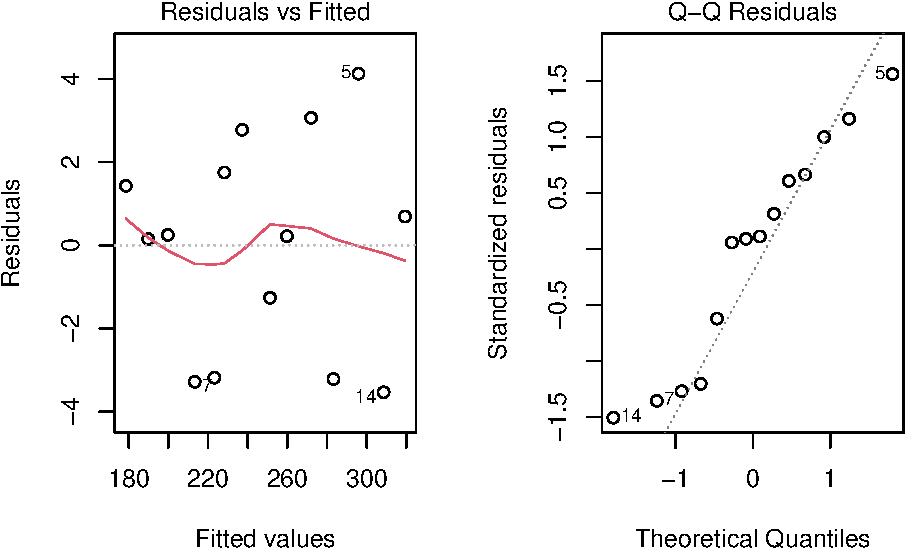
\includegraphics[keepaspectratio]{MultivariateStatisticalAnalysis_files/figure-latex/unnamed-chunk-9-1.pdf}}

\section{Estimación de parámetros}\label{estimaciuxf3n-de-paruxe1metros}

\textbf{Ejemplo (Montgomery, 2002):} : Un embotellador de bebidas gaseosas analiza las rutas de servicio de las máquinas expendedoras en su sistema de distribución. Le interesa predecir el tiempo necesario para que el representante de ruta atienda las máquinas expendedoras en una tienda.

Esta actividad de servicio consiste en abastecer la máquina con productos embotellados, y algo de mantenimiento o limpieza. El ingeniero industrial responsable del estudio ha sugerido que las dos variables más importantes que afectan el tiempo de entrega \(y\) son la cantidad de cajas de producto abastecido, \(x_1\), y la distancia caminada por el representante, \(x_2\).

El ingeniero ha reunido 25 observaciones de tiempo de entrega que se ven en la tabla siguiente. Se ajustará el modelo de regresión lineal multiple siguiente:

\[
y = \beta_0 + \beta_1 x_1 + \beta_2 x_2 +  \varepsilon
\]

\emph{Archivo: \texttt{refrescos.csv}}.

Base de datos

\begin{Shaded}
\begin{Highlighting}[]
\CommentTok{\# }
\NormalTok{datos }\OtherTok{\textless{}{-}} \FunctionTok{data.frame}\NormalTok{(}
  \AttributeTok{Observacion =} \DecValTok{1}\SpecialCharTok{:}\DecValTok{25}\NormalTok{,}
  \AttributeTok{y =} \FunctionTok{c}\NormalTok{(}\FloatTok{16.68}\NormalTok{, }\FloatTok{11.50}\NormalTok{, }\FloatTok{12.03}\NormalTok{, }\FloatTok{14.88}\NormalTok{, }\FloatTok{13.75}\NormalTok{,}
        \FloatTok{18.11}\NormalTok{, }\FloatTok{8.00}\NormalTok{, }\FloatTok{17.83}\NormalTok{, }\FloatTok{79.24}\NormalTok{, }\FloatTok{21.50}\NormalTok{,}
        \FloatTok{40.33}\NormalTok{, }\FloatTok{21.00}\NormalTok{, }\FloatTok{13.50}\NormalTok{, }\FloatTok{19.75}\NormalTok{, }\FloatTok{24.00}\NormalTok{,}
        \FloatTok{29.00}\NormalTok{, }\FloatTok{15.35}\NormalTok{, }\FloatTok{19.00}\NormalTok{, }\FloatTok{9.50}\NormalTok{, }\FloatTok{35.10}\NormalTok{,}
        \FloatTok{17.90}\NormalTok{, }\FloatTok{52.32}\NormalTok{, }\FloatTok{18.75}\NormalTok{, }\FloatTok{19.83}\NormalTok{, }\FloatTok{10.75}\NormalTok{),}
  \AttributeTok{x1 =} \FunctionTok{c}\NormalTok{(}\DecValTok{7}\NormalTok{, }\DecValTok{3}\NormalTok{, }\DecValTok{3}\NormalTok{, }\DecValTok{4}\NormalTok{, }\DecValTok{6}\NormalTok{,}
         \DecValTok{7}\NormalTok{, }\DecValTok{2}\NormalTok{, }\DecValTok{7}\NormalTok{, }\DecValTok{30}\NormalTok{, }\DecValTok{5}\NormalTok{,}
         \DecValTok{16}\NormalTok{, }\DecValTok{10}\NormalTok{, }\DecValTok{4}\NormalTok{, }\DecValTok{6}\NormalTok{, }\DecValTok{9}\NormalTok{,}
         \DecValTok{10}\NormalTok{, }\DecValTok{6}\NormalTok{, }\DecValTok{7}\NormalTok{, }\DecValTok{3}\NormalTok{, }\DecValTok{17}\NormalTok{,}
         \DecValTok{10}\NormalTok{, }\DecValTok{26}\NormalTok{, }\DecValTok{9}\NormalTok{, }\DecValTok{8}\NormalTok{, }\DecValTok{4}\NormalTok{),}
  \AttributeTok{x2 =} \FunctionTok{c}\NormalTok{(}\DecValTok{560}\NormalTok{, }\DecValTok{220}\NormalTok{, }\DecValTok{340}\NormalTok{, }\DecValTok{80}\NormalTok{, }\DecValTok{150}\NormalTok{,}
         \DecValTok{330}\NormalTok{, }\DecValTok{110}\NormalTok{, }\DecValTok{210}\NormalTok{, }\DecValTok{1460}\NormalTok{, }\DecValTok{605}\NormalTok{,}
         \DecValTok{688}\NormalTok{, }\DecValTok{215}\NormalTok{, }\DecValTok{255}\NormalTok{, }\DecValTok{462}\NormalTok{, }\DecValTok{448}\NormalTok{,}
         \DecValTok{776}\NormalTok{, }\DecValTok{200}\NormalTok{, }\DecValTok{132}\NormalTok{, }\DecValTok{36}\NormalTok{, }\DecValTok{770}\NormalTok{,}
         \DecValTok{140}\NormalTok{, }\DecValTok{810}\NormalTok{, }\DecValTok{450}\NormalTok{, }\DecValTok{635}\NormalTok{, }\DecValTok{150}\NormalTok{)}
\NormalTok{)}

\NormalTok{datos}
\end{Highlighting}
\end{Shaded}

\begin{verbatim}
##    Observacion     y x1   x2
## 1            1 16.68  7  560
## 2            2 11.50  3  220
## 3            3 12.03  3  340
## 4            4 14.88  4   80
## 5            5 13.75  6  150
## 6            6 18.11  7  330
## 7            7  8.00  2  110
## 8            8 17.83  7  210
## 9            9 79.24 30 1460
## 10          10 21.50  5  605
## 11          11 40.33 16  688
## 12          12 21.00 10  215
## 13          13 13.50  4  255
## 14          14 19.75  6  462
## 15          15 24.00  9  448
## 16          16 29.00 10  776
## 17          17 15.35  6  200
## 18          18 19.00  7  132
## 19          19  9.50  3   36
## 20          20 35.10 17  770
## 21          21 17.90 10  140
## 22          22 52.32 26  810
## 23          23 18.75  9  450
## 24          24 19.83  8  635
## 25          25 10.75  4  150
\end{verbatim}

Veamos un gráfico de dispersión de los datos. ¿Qué observamos?

\begin{Shaded}
\begin{Highlighting}[]
\FunctionTok{pairs}\NormalTok{(datos[}\SpecialCharTok{{-}}\DecValTok{1}\NormalTok{])}
\end{Highlighting}
\end{Shaded}

\pandocbounded{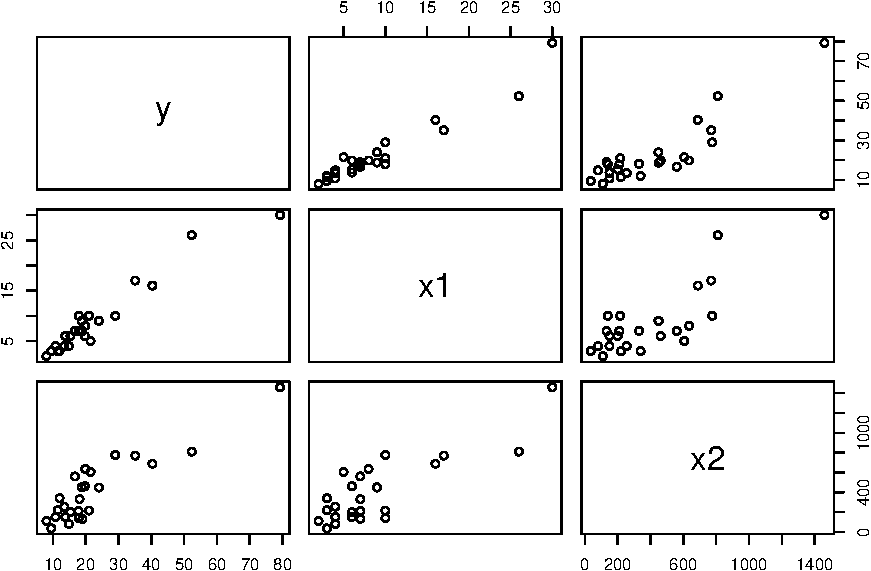
\includegraphics[keepaspectratio]{MultivariateStatisticalAnalysis_files/figure-latex/unnamed-chunk-11-1.pdf}}

\begin{enumerate}
\def\labelenumi{\arabic{enumi})}
\tightlist
\item
  Estimar \(\beta\)
\end{enumerate}

Primero, vamos a crear la matriz \(X\) y el vector \(y\).

Matrices

\begin{Shaded}
\begin{Highlighting}[]
\CommentTok{\# Columna de 1 para el intercepto}
\NormalTok{idv }\OtherTok{\textless{}{-}} \FunctionTok{rep}\NormalTok{(}\DecValTok{1}\NormalTok{, }\FunctionTok{nrow}\NormalTok{(datos))}
\CommentTok{\# Creamos matriz X}
\NormalTok{X }\OtherTok{\textless{}{-}} \FunctionTok{matrix}\NormalTok{(}\FunctionTok{c}\NormalTok{(idv,datos}\SpecialCharTok{$}\NormalTok{x1,datos}\SpecialCharTok{$}\NormalTok{x2),}\AttributeTok{nrow=}\DecValTok{25}\NormalTok{,}\AttributeTok{ncol=}\DecValTok{3}\NormalTok{)}
\CommentTok{\# Creamos el vector y}
\NormalTok{y }\OtherTok{\textless{}{-}} \FunctionTok{matrix}\NormalTok{(datos}\SpecialCharTok{$}\NormalTok{y, }\AttributeTok{nrow =} \DecValTok{25}\NormalTok{, }\AttributeTok{ncol =} \DecValTok{1}\NormalTok{)}
\end{Highlighting}
\end{Shaded}

Ya sabemos que nuestro estimador está dado por

\[
\hat{\beta} = (X'X)^{-1}X'y
\]

Entonces podemos encontrar el estimador.

Estimador beta

\begin{Shaded}
\begin{Highlighting}[]
\NormalTok{beta }\OtherTok{\textless{}{-}} \FunctionTok{solve}\NormalTok{(}\FunctionTok{t}\NormalTok{(X) }\SpecialCharTok{\%*\%}\NormalTok{ X) }\SpecialCharTok{\%*\%} \FunctionTok{t}\NormalTok{(X) }\SpecialCharTok{\%*\%}\NormalTok{ y}
\NormalTok{beta}
\end{Highlighting}
\end{Shaded}

\begin{verbatim}
##            [,1]
## [1,] 2.34123115
## [2,] 1.61590721
## [3,] 0.01438483
\end{verbatim}

Entonces el ajuste por el método de mínimos cuadrados, con los coeficientes de regresión que encontramos está dado por:

\(\hat{y} =\) 2.3412311 \(+\) 1.6159072 \(x_1\) \(+\) 1.6159072 \(x_2\)

Esto lo podemos hacer más rápido usando la función de \texttt{lm}. Construimos el modelo.

Modelo en R

\begin{Shaded}
\begin{Highlighting}[]
\NormalTok{M1 }\OtherTok{\textless{}{-}} \FunctionTok{lm}\NormalTok{(y }\SpecialCharTok{\textasciitilde{}}\NormalTok{ x1 }\SpecialCharTok{+}\NormalTok{ x2, datos)}
\NormalTok{M1 }
\end{Highlighting}
\end{Shaded}

\begin{verbatim}
## 
## Call:
## lm(formula = y ~ x1 + x2, data = datos)
## 
## Coefficients:
## (Intercept)           x1           x2  
##     2.34123      1.61591      0.01438
\end{verbatim}

¿Cómo accedemos a los valores del modelo?

Coeficientes

\begin{Shaded}
\begin{Highlighting}[]
\NormalTok{beta\_0 }\OtherTok{\textless{}{-}}\NormalTok{ M1}\SpecialCharTok{$}\NormalTok{coefficients[}\DecValTok{1}\NormalTok{]}
\NormalTok{beta\_1 }\OtherTok{\textless{}{-}}\NormalTok{ M1}\SpecialCharTok{$}\NormalTok{coefficients[}\DecValTok{2}\NormalTok{]}
\NormalTok{beta\_2 }\OtherTok{\textless{}{-}}\NormalTok{ M1}\SpecialCharTok{$}\NormalTok{coefficients[}\DecValTok{3}\NormalTok{]}
\end{Highlighting}
\end{Shaded}

Los valores son \(\beta_0=\) 2.3412311, \(\beta_1=\) 1.6159072 y \(\beta_2=\) 0.0143848.

\begin{enumerate}
\def\labelenumi{\arabic{enumi})}
\setcounter{enumi}{1}
\tightlist
\item
  Estimación de la varianza del error \(\sigma^2\)
\end{enumerate}

Ya tenemos que la suma de los cuadrados de los errores está dada por

\[ SSE = y'y - \hat{\beta}X'y\]

Sustituimos los valores que tenemos y obtemos el SSE.

SSE

\begin{Shaded}
\begin{Highlighting}[]
\NormalTok{SSE }\OtherTok{\textless{}{-}} \FunctionTok{t}\NormalTok{(y)}\SpecialCharTok{\%*\%}\NormalTok{ y }\SpecialCharTok{{-}} \FunctionTok{t}\NormalTok{(beta) }\SpecialCharTok{\%*\%} \FunctionTok{t}\NormalTok{(X) }\SpecialCharTok{\%*\%}\NormalTok{ y}
\NormalTok{SSE}
\end{Highlighting}
\end{Shaded}

\begin{verbatim}
##          [,1]
## [1,] 233.7317
\end{verbatim}

Y de está forma, podemos encontrar el estimador de \(\sigma^2\).

Estimador

\begin{Shaded}
\begin{Highlighting}[]
\NormalTok{varest }\OtherTok{\textless{}{-}}\NormalTok{ SSE }\SpecialCharTok{/}\NormalTok{ (}\FunctionTok{nrow}\NormalTok{(y) }\SpecialCharTok{{-}} \FunctionTok{nrow}\NormalTok{(beta))}
\NormalTok{varest}
\end{Highlighting}
\end{Shaded}

\begin{verbatim}
##          [,1]
## [1,] 10.62417
\end{verbatim}

Directo con las funciones de R, podemos acceder a los parámetros que se guardaron en el modelo que ya calculamos.

Resumen del modelo

\begin{Shaded}
\begin{Highlighting}[]
\FunctionTok{summary}\NormalTok{(M1)}
\end{Highlighting}
\end{Shaded}

\begin{verbatim}
## 
## Call:
## lm(formula = y ~ x1 + x2, data = datos)
## 
## Residuals:
##     Min      1Q  Median      3Q     Max 
## -5.7880 -0.6629  0.4364  1.1566  7.4197 
## 
## Coefficients:
##             Estimate Std. Error t value Pr(>|t|)    
## (Intercept) 2.341231   1.096730   2.135 0.044170 *  
## x1          1.615907   0.170735   9.464 3.25e-09 ***
## x2          0.014385   0.003613   3.981 0.000631 ***
## ---
## Signif. codes:  0 '***' 0.001 '**' 0.01 '*' 0.05 '.' 0.1 ' ' 1
## 
## Residual standard error: 3.259 on 22 degrees of freedom
## Multiple R-squared:  0.9596, Adjusted R-squared:  0.9559 
## F-statistic: 261.2 on 2 and 22 DF,  p-value: 4.687e-16
\end{verbatim}

Algunos de los parámetros almacenados en el modelo nos permiten obtener también el resultado previo.

Estimador

\begin{Shaded}
\begin{Highlighting}[]
\FunctionTok{sum}\NormalTok{(}\FunctionTok{residuals}\NormalTok{(M1)}\SpecialCharTok{\^{}}\DecValTok{2}\NormalTok{) }\SpecialCharTok{/} \FunctionTok{df.residual}\NormalTok{(M1)}
\end{Highlighting}
\end{Shaded}

\begin{verbatim}
## [1] 10.62417
\end{verbatim}

\subsection{Ejercicios}\label{ejercicios}

\textbf{Ejercicio 1:} Un analista hace un estudio químico y espera que el rendimiento de cierta sustancia se vea afectado por dos factores. Se realizan 17 experimentos cuyos datos se registran en el cuadro siguiente. Por experimentos similares, se sabe que los factores \(x_1\) y \(x_2\) no están relacionados; por ello, el analista decide utilizar un modelo de regresión lineal múltiple. Calcule el modelo de regresión y grafíquelo sobre las observaciones.

\emph{Archivo: est\_quimico.csv}

Datos Ejercicio 1

\begin{Shaded}
\begin{Highlighting}[]
\NormalTok{datos2 }\OtherTok{\textless{}{-}} \FunctionTok{data.frame}\NormalTok{(}
  \AttributeTok{Experimento =} \DecValTok{1}\SpecialCharTok{:}\DecValTok{17}\NormalTok{,}
  \AttributeTok{x1 =} \FunctionTok{c}\NormalTok{(}\FloatTok{41.9}\NormalTok{, }\FloatTok{43.4}\NormalTok{, }\FloatTok{43.9}\NormalTok{, }\FloatTok{44.5}\NormalTok{, }\FloatTok{47.3}\NormalTok{, }\FloatTok{47.5}\NormalTok{, }\FloatTok{47.9}\NormalTok{, }\FloatTok{50.2}\NormalTok{, }\FloatTok{52.8}\NormalTok{, }\FloatTok{53.2}\NormalTok{, }\FloatTok{56.7}\NormalTok{, }\FloatTok{57.0}\NormalTok{, }\FloatTok{63.5}\NormalTok{, }\FloatTok{64.3}\NormalTok{, }\FloatTok{71.1}\NormalTok{, }\FloatTok{77.0}\NormalTok{, }\FloatTok{77.8}\NormalTok{),}
  \AttributeTok{x2 =} \FunctionTok{c}\NormalTok{(}\FloatTok{29.1}\NormalTok{, }\FloatTok{29.3}\NormalTok{, }\FloatTok{29.5}\NormalTok{, }\FloatTok{29.7}\NormalTok{, }\FloatTok{29.9}\NormalTok{, }\FloatTok{30.3}\NormalTok{, }\FloatTok{30.5}\NormalTok{, }\FloatTok{30.7}\NormalTok{, }\FloatTok{30.8}\NormalTok{, }\FloatTok{30.9}\NormalTok{, }\FloatTok{31.5}\NormalTok{, }\FloatTok{31.7}\NormalTok{, }\FloatTok{31.9}\NormalTok{, }\FloatTok{32.0}\NormalTok{, }\FloatTok{32.1}\NormalTok{, }\FloatTok{32.5}\NormalTok{, }\FloatTok{32.9}\NormalTok{),}
  \AttributeTok{y  =} \FunctionTok{c}\NormalTok{(}\FloatTok{251.3}\NormalTok{, }\FloatTok{251.3}\NormalTok{, }\FloatTok{248.3}\NormalTok{, }\FloatTok{267.5}\NormalTok{, }\FloatTok{273.0}\NormalTok{, }\FloatTok{276.5}\NormalTok{, }\FloatTok{270.3}\NormalTok{, }\FloatTok{274.9}\NormalTok{, }\FloatTok{285.0}\NormalTok{, }\FloatTok{290.0}\NormalTok{, }\FloatTok{297.0}\NormalTok{, }\FloatTok{302.5}\NormalTok{, }\FloatTok{304.5}\NormalTok{, }\FloatTok{309.3}\NormalTok{, }\FloatTok{321.7}\NormalTok{, }\FloatTok{330.7}\NormalTok{, }\FloatTok{349.0}\NormalTok{)}
\NormalTok{)}

\NormalTok{datos2}
\end{Highlighting}
\end{Shaded}

\begin{verbatim}
##    Experimento   x1   x2     y
## 1            1 41.9 29.1 251.3
## 2            2 43.4 29.3 251.3
## 3            3 43.9 29.5 248.3
## 4            4 44.5 29.7 267.5
## 5            5 47.3 29.9 273.0
## 6            6 47.5 30.3 276.5
## 7            7 47.9 30.5 270.3
## 8            8 50.2 30.7 274.9
## 9            9 52.8 30.8 285.0
## 10          10 53.2 30.9 290.0
## 11          11 56.7 31.5 297.0
## 12          12 57.0 31.7 302.5
## 13          13 63.5 31.9 304.5
## 14          14 64.3 32.0 309.3
## 15          15 71.1 32.1 321.7
## 16          16 77.0 32.5 330.7
## 17          17 77.8 32.9 349.0
\end{verbatim}

\textbf{Ejercicio 2:} Repetir el ejemplo con los datos \texttt{datasets::trees} de R que proporciona mediciones
del diámetro, altura y volumen de madera en 31 cerezos negros talados.

\textbf{Ejercicio 3:} Subir a Github los dos ejercicios previos tanto con solución en R como en Python. Comparar las funciones. Ventajas y desventajas de ambas.

\section{Pruebas de Hipótesis}\label{pruebas-de-hipuxf3tesis}

Cuando revisamos el \texttt{summary} del modelo, nos arroja si son significativas o no y a que nivel de significancia las variables que estamos considerando. Veamos el siguiente ejemplo.

\subsection{Prueba de la significancia de la regresión}\label{prueba-de-la-significancia-de-la-regresiuxf3n}

\textbf{Ejemplo:} Con los datos del embotellador de bebidas gaseosas, se probará la significancia de la regresión.

Sumas de Cuadrados

\begin{Shaded}
\begin{Highlighting}[]
\NormalTok{SCT }\OtherTok{\textless{}{-}} \FunctionTok{t}\NormalTok{(y) }\SpecialCharTok{\%*\%}\NormalTok{ y }\SpecialCharTok{{-}}  \FunctionTok{sum}\NormalTok{(y)}\SpecialCharTok{**}\DecValTok{2} \SpecialCharTok{/} \FunctionTok{nrow}\NormalTok{(datos)}
\NormalTok{SCT}
\end{Highlighting}
\end{Shaded}

\begin{verbatim}
##          [,1]
## [1,] 5784.543
\end{verbatim}

\begin{Shaded}
\begin{Highlighting}[]
\NormalTok{SCE }\OtherTok{\textless{}{-}} \FunctionTok{t}\NormalTok{(beta) }\SpecialCharTok{\%*\%} \FunctionTok{t}\NormalTok{(X) }\SpecialCharTok{\%*\%}\NormalTok{ y }\SpecialCharTok{{-}} \FunctionTok{sum}\NormalTok{(y)}\SpecialCharTok{**}\DecValTok{2} \SpecialCharTok{/} \FunctionTok{nrow}\NormalTok{(datos)}
\NormalTok{SCE}
\end{Highlighting}
\end{Shaded}

\begin{verbatim}
##          [,1]
## [1,] 5550.811
\end{verbatim}

\begin{Shaded}
\begin{Highlighting}[]
\NormalTok{SSE }\OtherTok{\textless{}{-}}\NormalTok{ SCT }\SpecialCharTok{{-}}\NormalTok{ SCE}
\NormalTok{SSE}
\end{Highlighting}
\end{Shaded}

\begin{verbatim}
##          [,1]
## [1,] 233.7317
\end{verbatim}

Para probar

\[H_0 : \beta_1 = \beta_2=0\]

se calcula el estadístico:

Estadístico F

\begin{Shaded}
\begin{Highlighting}[]
\NormalTok{F0 }\OtherTok{\textless{}{-}}\NormalTok{ (SCE }\SpecialCharTok{/}\NormalTok{ (}\FunctionTok{ncol}\NormalTok{(X) }\SpecialCharTok{{-}} \DecValTok{1}\NormalTok{)) }\SpecialCharTok{/}\NormalTok{ (SSE }\SpecialCharTok{/}\NormalTok{ (}\FunctionTok{nrow}\NormalTok{(X) }\SpecialCharTok{{-}}\NormalTok{ (}\FunctionTok{ncol}\NormalTok{(X) }\SpecialCharTok{{-}}\DecValTok{1}\NormalTok{) }\SpecialCharTok{{-}} \DecValTok{1}\NormalTok{))}
\NormalTok{F0}
\end{Highlighting}
\end{Shaded}

\begin{verbatim}
##          [,1]
## [1,] 261.2351
\end{verbatim}

Como el valor de \(F_0\) es mayor que el valor tabulado de \(F_{\alpha;p,n-p-1}=F_{0.05;2;22}=3.44\), se rechaza \(H_0\). Lo cual implica qye el tiempo de entrega depende del volumen de entrega y/o de la distancia.

Ahora, usando los modelos que ya calculamos.

Sumas de cuadrados

\begin{Shaded}
\begin{Highlighting}[]
\NormalTok{SCT.m}\OtherTok{\textless{}{-}}\FunctionTok{sum}\NormalTok{((datos}\SpecialCharTok{$}\NormalTok{y}\SpecialCharTok{{-}}\FunctionTok{mean}\NormalTok{(datos}\SpecialCharTok{$}\NormalTok{y))}\SpecialCharTok{\^{}}\DecValTok{2}\NormalTok{)}
\NormalTok{SCT.m}
\end{Highlighting}
\end{Shaded}

\begin{verbatim}
## [1] 5784.543
\end{verbatim}

\begin{Shaded}
\begin{Highlighting}[]
\NormalTok{SCE.m }\OtherTok{\textless{}{-}}\FunctionTok{sum}\NormalTok{((M1}\SpecialCharTok{$}\NormalTok{fitted}\SpecialCharTok{{-}}\FunctionTok{mean}\NormalTok{(datos}\SpecialCharTok{$}\NormalTok{y))}\SpecialCharTok{\^{}}\DecValTok{2}\NormalTok{)}
\NormalTok{SCE.m}
\end{Highlighting}
\end{Shaded}

\begin{verbatim}
## [1] 5550.811
\end{verbatim}

\begin{Shaded}
\begin{Highlighting}[]
\NormalTok{SSE.m }\OtherTok{\textless{}{-}}\FunctionTok{sum}\NormalTok{(M1}\SpecialCharTok{$}\NormalTok{residuals}\SpecialCharTok{\^{}}\DecValTok{2}\NormalTok{)}
\NormalTok{SSE.m}
\end{Highlighting}
\end{Shaded}

\begin{verbatim}
## [1] 233.7317
\end{verbatim}

Grados de libertad

\begin{Shaded}
\begin{Highlighting}[]
\NormalTok{n}\OtherTok{\textless{}{-}}\FunctionTok{nrow}\NormalTok{(y)}
\NormalTok{n}
\end{Highlighting}
\end{Shaded}

\begin{verbatim}
## [1] 25
\end{verbatim}

\begin{Shaded}
\begin{Highlighting}[]
\NormalTok{GLT}\OtherTok{\textless{}{-}}\NormalTok{ n}\DecValTok{{-}1}
\NormalTok{GLT}
\end{Highlighting}
\end{Shaded}

\begin{verbatim}
## [1] 24
\end{verbatim}

\begin{Shaded}
\begin{Highlighting}[]
\NormalTok{GLRes}\OtherTok{\textless{}{-}} \FunctionTok{df.residual}\NormalTok{(M1)}
\NormalTok{GLRes}
\end{Highlighting}
\end{Shaded}

\begin{verbatim}
## [1] 22
\end{verbatim}

\begin{Shaded}
\begin{Highlighting}[]
\NormalTok{GLR}\OtherTok{\textless{}{-}}\NormalTok{ GLT}\SpecialCharTok{{-}}\NormalTok{GLRes}
\NormalTok{GLR}
\end{Highlighting}
\end{Shaded}

\begin{verbatim}
## [1] 2
\end{verbatim}

Cuadrados medios

\begin{Shaded}
\begin{Highlighting}[]
\NormalTok{CMR }\OtherTok{\textless{}{-}}\NormalTok{ SCE }\SpecialCharTok{/}\NormalTok{GLR}
\NormalTok{CMR}
\end{Highlighting}
\end{Shaded}

\begin{verbatim}
##          [,1]
## [1,] 2775.405
\end{verbatim}

\begin{Shaded}
\begin{Highlighting}[]
\NormalTok{CMRes }\OtherTok{\textless{}{-}}\NormalTok{ SSE }\SpecialCharTok{/}\NormalTok{ GLRes}
\NormalTok{CMRes}
\end{Highlighting}
\end{Shaded}

\begin{verbatim}
##          [,1]
## [1,] 10.62417
\end{verbatim}

Estadístico F\_0

\begin{Shaded}
\begin{Highlighting}[]
\NormalTok{F0 }\OtherTok{\textless{}{-}}\NormalTok{ CMR}\SpecialCharTok{/}\NormalTok{CMRes}
\NormalTok{F0}
\end{Highlighting}
\end{Shaded}

\begin{verbatim}
##          [,1]
## [1,] 261.2351
\end{verbatim}

p-valor

\begin{Shaded}
\begin{Highlighting}[]
\NormalTok{pv }\OtherTok{\textless{}{-}} \DecValTok{1} \SpecialCharTok{{-}} \FunctionTok{pf}\NormalTok{(F0, GLR,GLRes)}
\NormalTok{pv}
\end{Highlighting}
\end{Shaded}

\begin{verbatim}
##              [,1]
## [1,] 4.440892e-16
\end{verbatim}

Valor tabulado de F

\begin{Shaded}
\begin{Highlighting}[]
\NormalTok{alpha }\OtherTok{\textless{}{-}} \FloatTok{0.05}\NormalTok{; df1 }\OtherTok{\textless{}{-}} \DecValTok{2}\NormalTok{; df2 }\OtherTok{\textless{}{-}} \DecValTok{22}
\NormalTok{F\_crit }\OtherTok{\textless{}{-}} \FunctionTok{qf}\NormalTok{(}\DecValTok{1} \SpecialCharTok{{-}}\NormalTok{ alpha, df1, df2)}
\NormalTok{F\_crit}
\end{Highlighting}
\end{Shaded}

\begin{verbatim}
## [1] 3.443357
\end{verbatim}

\subsection{Pruebas sobre coeficientes individuales de regresión}\label{pruebas-sobre-coeficientes-individuales-de-regresiuxf3n}

\textbf{Ejemplo:} Usando los datos del embotellador de bebidas gaseosas, se desea evaluar la importancia de la variable regresora \emph{distancia} (\(x_2\)) dado que el regresor \emph{cajas} (\(x_1\)) está en el modelo.

Estadístico t\_0

\begin{Shaded}
\begin{Highlighting}[]
\NormalTok{C22 }\OtherTok{\textless{}{-}} \FunctionTok{solve}\NormalTok{(}\FunctionTok{t}\NormalTok{(X) }\SpecialCharTok{\%*\%}\NormalTok{ X)[}\DecValTok{3}\NormalTok{,}\DecValTok{3}\NormalTok{]}
\NormalTok{C22}
\end{Highlighting}
\end{Shaded}

\begin{verbatim}
## [1] 1.228745e-06
\end{verbatim}

\begin{Shaded}
\begin{Highlighting}[]
\NormalTok{t0 }\OtherTok{\textless{}{-}}\NormalTok{ beta\_2 }\SpecialCharTok{/} \FunctionTok{sqrt}\NormalTok{(varest }\SpecialCharTok{*}\NormalTok{ C22)}
\NormalTok{t0}
\end{Highlighting}
\end{Shaded}

\begin{verbatim}
##          [,1]
## [1,] 3.981313
\end{verbatim}

\begin{Shaded}
\begin{Highlighting}[]
\DocumentationTok{\#\# t tabulado con confianza 95\% y 22 grados de libertad}
\NormalTok{tt }\OtherTok{\textless{}{-}} \FunctionTok{qt}\NormalTok{(}\AttributeTok{p =} \FloatTok{0.95} \SpecialCharTok{+} \FloatTok{0.05}\SpecialCharTok{/}\DecValTok{2}\NormalTok{, }\AttributeTok{df =} \DecValTok{22}\NormalTok{, }\AttributeTok{lower.tail =} \ConstantTok{TRUE}\NormalTok{)}
\NormalTok{tt}
\end{Highlighting}
\end{Shaded}

\begin{verbatim}
## [1] 2.073873
\end{verbatim}

Usando el modelo que ya tenemos calculado \texttt{M1} podemos obtener estos mismos resultados de la siguiente forma.

Prueba sobre coeficientes

\begin{Shaded}
\begin{Highlighting}[]
\FunctionTok{summary}\NormalTok{(M1)}
\end{Highlighting}
\end{Shaded}

\begin{verbatim}
## 
## Call:
## lm(formula = y ~ x1 + x2, data = datos)
## 
## Residuals:
##     Min      1Q  Median      3Q     Max 
## -5.7880 -0.6629  0.4364  1.1566  7.4197 
## 
## Coefficients:
##             Estimate Std. Error t value Pr(>|t|)    
## (Intercept) 2.341231   1.096730   2.135 0.044170 *  
## x1          1.615907   0.170735   9.464 3.25e-09 ***
## x2          0.014385   0.003613   3.981 0.000631 ***
## ---
## Signif. codes:  0 '***' 0.001 '**' 0.01 '*' 0.05 '.' 0.1 ' ' 1
## 
## Residual standard error: 3.259 on 22 degrees of freedom
## Multiple R-squared:  0.9596, Adjusted R-squared:  0.9559 
## F-statistic: 261.2 on 2 and 22 DF,  p-value: 4.687e-16
\end{verbatim}

\section{Intervalos de confianza}\label{intervalos-de-confianza}

\subsection{Intervalos de confianza en los coeficientes de regresión}\label{intervalos-de-confianza-en-los-coeficientes-de-regresiuxf3n}

\textbf{Ejemplo:} Usando los datos del embotellador de bebidas gaseosas, queremos calcular el intervalo de confianza del 95\% para \(\beta_1\). Recordemos que el estimador puntual de \(\beta_1\) es 1.6159072.

Intervalo de confianza

\begin{Shaded}
\begin{Highlighting}[]
\NormalTok{C11 }\OtherTok{\textless{}{-}} \FunctionTok{solve}\NormalTok{(}\FunctionTok{t}\NormalTok{(X) }\SpecialCharTok{\%*\%}\NormalTok{ X)[}\DecValTok{2}\NormalTok{,}\DecValTok{2}\NormalTok{]}

\NormalTok{izq }\OtherTok{\textless{}{-}}\NormalTok{ beta\_1 }\SpecialCharTok{{-}}\NormalTok{ tt }\SpecialCharTok{*} \FunctionTok{sqrt}\NormalTok{(varest}\SpecialCharTok{*}\NormalTok{C11)}
\NormalTok{izq}
\end{Highlighting}
\end{Shaded}

\begin{verbatim}
##          [,1]
## [1,] 1.261825
\end{verbatim}

\begin{Shaded}
\begin{Highlighting}[]
\NormalTok{der }\OtherTok{\textless{}{-}}\NormalTok{ beta\_1 }\SpecialCharTok{+}\NormalTok{ tt }\SpecialCharTok{*} \FunctionTok{sqrt}\NormalTok{(varest}\SpecialCharTok{*}\NormalTok{C11)}
\NormalTok{der}
\end{Highlighting}
\end{Shaded}

\begin{verbatim}
##         [,1]
## [1,] 1.96999
\end{verbatim}

\subsection{Intervalo de confianza de la respuesta media}\label{intervalo-de-confianza-de-la-respuesta-media}

\textbf{Ejemplo:} El embotellador de bebidas gaseosas quiere establecer un intervalo de confianza del 95\% para el tiempo medio de entrega para una tienda donde se requieren \(x_1=8\) cajas y la distancia es de \(x_2=275\) pies.

Nuestro vector \(X_0\) está dado por:

X0

\begin{Shaded}
\begin{Highlighting}[]
\NormalTok{X0 }\OtherTok{\textless{}{-}} \FunctionTok{matrix}\NormalTok{(}\FunctionTok{c}\NormalTok{(}\DecValTok{1}\NormalTok{, }\DecValTok{8}\NormalTok{, }\DecValTok{275}\NormalTok{), }\AttributeTok{nrow =} \DecValTok{3}\NormalTok{)}
\NormalTok{X0}
\end{Highlighting}
\end{Shaded}

\begin{verbatim}
##      [,1]
## [1,]    1
## [2,]    8
## [3,]  275
\end{verbatim}

El valor ajustado en ese punto es:

Valor ajustado

\begin{Shaded}
\begin{Highlighting}[]
\NormalTok{y0 }\OtherTok{\textless{}{-}} \FunctionTok{t}\NormalTok{(X0) }\SpecialCharTok{\%*\%}\NormalTok{ beta}
\NormalTok{y0}
\end{Highlighting}
\end{Shaded}

\begin{verbatim}
##          [,1]
## [1,] 19.22432
\end{verbatim}

La varianza de \(\hat{y_0}\)

Varianza

\begin{Shaded}
\begin{Highlighting}[]
\NormalTok{var\_y0 }\OtherTok{\textless{}{-}}\NormalTok{ varest }\SpecialCharTok{*} \FunctionTok{t}\NormalTok{(X0) }\SpecialCharTok{\%*\%} \FunctionTok{solve}\NormalTok{(}\FunctionTok{t}\NormalTok{(X) }\SpecialCharTok{\%*\%}\NormalTok{ X) }\SpecialCharTok{\%*\%}\NormalTok{ X0}
\NormalTok{var\_y0}
\end{Highlighting}
\end{Shaded}

\begin{verbatim}
##           [,1]
## [1,] 0.5734134
\end{verbatim}

Entonces el intervalo de confianza en este punto es:

Intervalo de confianza

\begin{Shaded}
\begin{Highlighting}[]
\NormalTok{l\_izq }\OtherTok{\textless{}{-}}\NormalTok{ y0 }\SpecialCharTok{{-}}\NormalTok{ tt }\SpecialCharTok{*} \FunctionTok{sqrt}\NormalTok{(var\_y0) }
\NormalTok{l\_izq}
\end{Highlighting}
\end{Shaded}

\begin{verbatim}
##         [,1]
## [1,] 17.6539
\end{verbatim}

\begin{Shaded}
\begin{Highlighting}[]
\NormalTok{l\_der }\OtherTok{\textless{}{-}}\NormalTok{ y0 }\SpecialCharTok{+}\NormalTok{ tt }\SpecialCharTok{*} \FunctionTok{sqrt}\NormalTok{(var\_y0) }
\NormalTok{l\_der}
\end{Highlighting}
\end{Shaded}

\begin{verbatim}
##          [,1]
## [1,] 20.79474
\end{verbatim}

\textbf{Ejemplo: } Usaremos el conjunto de datos \texttt{data("marketing")} que contiene 200 observaciones de un experimento publicitario que evalúa el impacto de tres medios de anuncio en las ventas. Para cada observación se registran los presupuestos de publicidad (en miles de dólares) y las ventas obtenidas.
Variables:

\begin{itemize}
\tightlist
\item
  \texttt{youtube}: presupuesto invertido en anuncios de YouTube (miles de USD).
\item
  \texttt{facebook}: presupuesto invertido en Facebook (miles de USD).
\item
  \texttt{newspaper}: presupuesto invertido en prensa escrita (miles de USD).
\item
  \texttt{sales}: ventas registradas (variable respuesta).
\end{itemize}

Cargamos los datos:

\begin{Shaded}
\begin{Highlighting}[]
\FunctionTok{library}\NormalTok{(datarium)}
\FunctionTok{data}\NormalTok{(}\StringTok{"marketing"}\NormalTok{)}
\end{Highlighting}
\end{Shaded}

Exploramos rápidamente la base para ver qué variables contiene y la dimensión:

\begin{Shaded}
\begin{Highlighting}[]
\FunctionTok{str}\NormalTok{(marketing)}
\end{Highlighting}
\end{Shaded}

\begin{verbatim}
## 'data.frame':    200 obs. of  4 variables:
##  $ youtube  : num  276.1 53.4 20.6 181.8 217 ...
##  $ facebook : num  45.4 47.2 55.1 49.6 13 ...
##  $ newspaper: num  83 54.1 83.2 70.2 70.1 ...
##  $ sales    : num  26.5 12.5 11.2 22.2 15.5 ...
\end{verbatim}

\begin{Shaded}
\begin{Highlighting}[]
\CommentTok{\#?marketing}
\end{Highlighting}
\end{Shaded}

Ajustamos un modelo lineal que incluya todas las variables, es decir,

\(sales=\beta_0+\beta_1 youtube+\beta_2 facebook+ \beta_3 newspaper+\epsilon\)

Modelo marketing

\begin{Shaded}
\begin{Highlighting}[]
\NormalTok{modelo1}\OtherTok{\textless{}{-}}\FunctionTok{lm}\NormalTok{(sales}\SpecialCharTok{\textasciitilde{}}\NormalTok{youtube}\SpecialCharTok{+}\NormalTok{facebook}\SpecialCharTok{+}\NormalTok{newspaper,}\AttributeTok{data=}\NormalTok{marketing)}
\FunctionTok{summary}\NormalTok{(modelo1)}
\end{Highlighting}
\end{Shaded}

\begin{verbatim}
## 
## Call:
## lm(formula = sales ~ youtube + facebook + newspaper, data = marketing)
## 
## Residuals:
##      Min       1Q   Median       3Q      Max 
## -10.5932  -1.0690   0.2902   1.4272   3.3951 
## 
## Coefficients:
##              Estimate Std. Error t value Pr(>|t|)    
## (Intercept)  3.526667   0.374290   9.422   <2e-16 ***
## youtube      0.045765   0.001395  32.809   <2e-16 ***
## facebook     0.188530   0.008611  21.893   <2e-16 ***
## newspaper   -0.001037   0.005871  -0.177     0.86    
## ---
## Signif. codes:  0 '***' 0.001 '**' 0.01 '*' 0.05 '.' 0.1 ' ' 1
## 
## Residual standard error: 2.023 on 196 degrees of freedom
## Multiple R-squared:  0.8972, Adjusted R-squared:  0.8956 
## F-statistic: 570.3 on 3 and 196 DF,  p-value: < 2.2e-16
\end{verbatim}

¿Qué se puede decir sobre la significancia de la variable \(newspaper\)?

Veamos qué ocurre con el modelo al eliminar la variable \(newspaper\)

Modelo marketing 2

\begin{Shaded}
\begin{Highlighting}[]
\NormalTok{modelo2}\OtherTok{\textless{}{-}}\FunctionTok{lm}\NormalTok{(sales}\SpecialCharTok{\textasciitilde{}}\NormalTok{facebook}\SpecialCharTok{+}\NormalTok{youtube,}\AttributeTok{data=}\NormalTok{marketing)}
\FunctionTok{summary}\NormalTok{(modelo2)}
\end{Highlighting}
\end{Shaded}

\begin{verbatim}
## 
## Call:
## lm(formula = sales ~ facebook + youtube, data = marketing)
## 
## Residuals:
##      Min       1Q   Median       3Q      Max 
## -10.5572  -1.0502   0.2906   1.4049   3.3994 
## 
## Coefficients:
##             Estimate Std. Error t value Pr(>|t|)    
## (Intercept)  3.50532    0.35339   9.919   <2e-16 ***
## facebook     0.18799    0.00804  23.382   <2e-16 ***
## youtube      0.04575    0.00139  32.909   <2e-16 ***
## ---
## Signif. codes:  0 '***' 0.001 '**' 0.01 '*' 0.05 '.' 0.1 ' ' 1
## 
## Residual standard error: 2.018 on 197 degrees of freedom
## Multiple R-squared:  0.8972, Adjusted R-squared:  0.8962 
## F-statistic: 859.6 on 2 and 197 DF,  p-value: < 2.2e-16
\end{verbatim}

Lo que sigue, es hacer pruebas de hipótesis tanto en las variables como en los coeficientes de regresión.

\textbf{Ejercicio 1:} Realizar las pruebas de hipótesis sobre la significancia de la regresión y sobre los coeficientes. Encontrar los intervalos de confianza respectivos del 95\%.
Para una tienda con presupuestos:
\(youtube = 150\), \(facebook = 30\), \(newspaper=20\) (en miles de USD):
(a) Calcula el intervalo de confianza del 95\% para la media de ventas \(\mathbb{E}(sales | X_0)\).
(b) Calcula el intervalo de predicción del 95\% para una nueva observación de ventas.
(c) Comenta la diferencia entre ambos intervalos.
Subir respuesta y explicación de sus resultados a github.

\section{Ejercicios}\label{ejercicios-1}

\textbf{Ejercicio 1:} Para los datos de la \href{https://github.com/HaydeePeruyero/MultivariateStatisticalAnalysis/tree/main/data/Liga_nacional_de_futbol.csv}{Liga Nacional de Fútbol}

\begin{enumerate}
\def\labelenumi{\alph{enumi})}
\item
  Ajustar un modelo de regresión lineal múltiple que relacione la cantidad de juegos ganados con las yardas por aire del equipo (\(x_2\)), el porcentaje de jugadas por tierra (\(x_7\)) y las yardas por tierra del contrario (\(x_8\)).
\item
  Formar la tabla de análisis de varianza y probar la significancia de la regresión.
\item
  Calcular el estadístico \emph{t} para probar las hipótesis \(H_0 : \beta_2 = 0\), \(H_0 : \beta_7 = 0\) y \(H_0 : \beta_8 = 0\). ¿Qué conclusiones se pueden sacar acerca del papel de las variables \(x_2\), \(x_7\) y \(x_8\) en el modelo?
\item
  Calcular \(R^2\) y \(R^2_{adj}\) para este modelo.
\item
  Trazar una gráfica de probabilidad normal de los residuales. ¿Parece haber algún problema con la hipótesis de normalidad?
\item
  Trazar e interpretar una gráfica de los residuales en función de la respuesta predicha.
\item
  Trazar las gráficas de los residuales en función de cada una de las variables regresoras. ¿Implican esas gráficas que se especificó en forma correcta el regresor?
\item
  Calcular un intervalo de confianza de \(95\%\) para \(\beta_7\) y un intervalo de confianza de \(95\%\) para la cantidad media de juegos ganados por un equipo cuando \(x_2 = 2300\), \(x_7 = 56\) y \(x_8 = 2100\).
\item
  Ajustar un modelo a esos datos, usando solo \(x_7\) y \(x_8\) como regresores y probar la significancia de la regresión.
\item
  Calcular \(R^2\) y \(R^2_{adj}\). Compararlos con los resultados del modelo anterior.
\item
  Calcular un intervalo de confianza de \(95\%\) para \(\beta_7\). También, un intervalo de confianza de \(95\%\) para la cantidad media de juegos ganados por un equipo cuando \(x_7 = 56\) y \(x_8 = 2100\). Comparar las longitudes de esos intervalos de confianza con las longitudes de los correspondientes al modelo anterior.
\item
  ¿Qué conclusiones se pueden sacar de este problema, acerca de las consecuencias de omitir un regresor importante de un modelo?
\end{enumerate}

\textbf{Ejericio 2:} Véase los datos de \href{https://github.com/HaydeePeruyero/MultivariateStatisticalAnalysis/tree/main/data/Rendimiento_de_gasolina.csv}{rendimiento de gasolina}.

\begin{enumerate}
\def\labelenumi{\alph{enumi})}
\item
  Ajustar un modelo de regresión lineal múltiple que relacione el rendimiento de la gasolina \emph{y}, en millas por galón, la cilindrada del motor (\(x_1\)) y la cantidad de gargantas del carburador (\(x_6\)).
\item
  Formar la tabla de análisis de varianza y probar la significancia de la regresión.
\item
  Calcular \(R^2\) y \(R^2_{adj}\) para este modelo. Compararlas con las \(R^2\) y \(R^2_{adj}\) Ajustado para el modelo de regresión lineal simple, que relaciona las millas con la cilindrada.
\item
  Determinar un intervalo de confianza para \(\beta_1\).
\item
  Determinar un intervalo de confianza de \(95\%\) para el rendimiento promedio de la gasolina, cuando \(x_1 = 225 pulg^3\) y \(x_6 = 2\) gargantas.
\item
  Determinar un intervalo de predicción de \(95\%\) para una nueva observación de rendimiento de gasolina, cuando \(x_1 = 225 pulg^3\) y \(x_6 = 2\) gargantas.
\item
  Considerar el modelo de regresión lineal simple, que relaciona las millas con la cilindrada. Construir un intervalo de confianza de \(95\%\) para el rendimiento promedio de la gasolina y un intervalo de predicción para el rendimiento, cuando \(x_1 = 225 pulg^3\). Comparar las longitudes de estos intervalos con los intervalos obtenidos en los dos incisos anteriores. ¿Tiene ventajas agregar \(x_6\) al modelo?
\item
  Trazar una gráfica de probabilidad normal de los residuales. ¿Parece haber algún problema con la hipótesis de normalidad?
\item
  Trazar e interpretar una gráfica de los residuales en función de la respuesta predicha.
\item
  Trazar las gráficas de los residuales en función de cada una de las variables regresoras. ¿Implican esas gráficas que se especificó en forma correcta el regresor?
\end{enumerate}

\chapter{Análisis de Componentes Principales}\label{anuxe1lisis-de-componentes-principales}

\chapter{Análisis Factorial}\label{anuxe1lisis-factorial}

\chapter{Análisis de Conglomerados}\label{anuxe1lisis-de-conglomerados}

\chapter{Análisis de Discriminante}\label{anuxe1lisis-de-discriminante}

\chapter{Apéndices}\label{apuxe9ndices}

\section{Introducción a R}\label{introducciuxf3n-a-r}

\begin{itemize}
\item
  Tutorial de RMarkdown: \href{https://github.com/HaydeePeruyero/Rmarkdown_and_LaTeX/blob/main/ejemplo.Rmd}{Link}
\item
  Tutorial Manejo de Proyectos: \href{https://haydeeperuyero.github.io/Seminario_Estadistica/manejo-de-proyectos.html}{Link}
\end{itemize}

\section{Git + Github}\label{git-github}

\begin{itemize}
\tightlist
\item
  Conectar R con Git y Github: \href{https://r-ladies-morelia.github.io/blog/conectar/}{Link}
\end{itemize}

\section{Gráficas Multivariadas}\label{gruxe1ficas-multivariadas}

\section{Escalas de Medición}\label{escalas-de-mediciuxf3n}

\section{Valores Faltantes}\label{valores-faltantes}

  \bibliography{book.bib,packages.bib}

\end{document}
